% Proyecto para Overleaf: seleccionar pdfLaTeX.
% Adjuntar figuras/boxplot_cambios.png y figuras/boxplot_lenguajes.png.
% No requiere CSV ni bibliografía externa.
% Azul: correcciones del texto de primera_version.tex.
% Negro: contenido conservado y agregaciones de la Etapa 2.
% Datos: GHAW-H, revisión 9ccc840bd7e96fd90db3a16548d5482c2833c47d.
% Los dos boxplots contienen estadísticas y observaciones atípicas reales.
\documentclass[conference,a4paper]{IEEEtran}
\usepackage[utf8]{inputenc}
\usepackage[T1]{fontenc}
\usepackage[spanish]{babel}
\usepackage{cite}
\usepackage{amsmath,booktabs,array,xcolor}
\usepackage{graphicx}
\usepackage[hidelinks]{hyperref}
\definecolor{correccion}{RGB}{0,70,170}
\newcommand{\corr}[1]{{\color{correccion}#1}}
% Sustituir estos dos campos cuando se publique el paquete propio.
\newcommand{\GitHubReplica}{\textit{pendiente de publicación}}
\newcommand{\ZenodoReplica}{\textit{pendiente de publicación}}
\setlength{\textfloatsep}{8pt plus 2pt minus 2pt}
\setlength{\floatsep}{7pt plus 2pt minus 2pt}
\setlength{\intextsep}{7pt plus 2pt minus 2pt}
\renewcommand{\refname}{Referencias}
\pagestyle{plain}

\begin{document}
\title{\corr{Mantenimiento de archivos Markdown en GitHub Agentic Workflows: un estudio empírico de su evolución con GHAW-H}}
\author{\IEEEauthorblockN{Francisco Barrozo}
\IEEEauthorblockA{\textit{Facultad de Ingeniería y Ciencias (FICA)}\\
\textit{Universidad de La Frontera}\\Temuco, Chile\\f.barrozo02@ufromail.cl}
\and
\IEEEauthorblockN{Antonia Paredes}
\IEEEauthorblockA{\textit{Facultad de Ingeniería y Ciencias (FICA)}\\
\textit{Universidad de La Frontera}\\Temuco, Chile\\a.paredes03@ufromail.cl}}
\maketitle

\begin{abstract}
\corr{Los archivos Markdown de GitHub Agentic Workflows contienen instrucciones y configuración que requieren mantenimiento junto al repositorio. El objetivo es caracterizar la recurrencia y magnitud de sus cambios textuales y examinar su variación entre contextos de lenguaje principal.}
Se analizaron las cinco tablas de GHAW-H: 262 repositorios, 604 historias y 2.820 versiones. En 2.216 transiciones enlazadas, 954 cambian líneas del cuerpo Markdown y 1.260 modifican solamente la configuración YAML. Los cambios efectivos del cuerpo presentan una mediana de 11 líneas añadidas más eliminadas. Los boxplots muestran dispersión y valores atípicos, mientras la comparación por lenguaje evidencia diferencias condicionadas por plantillas e importaciones. Estos resultados describen mantenimiento textual observable; no estiman esfuerzo humano, calidad de ejecución ni efectos causales del lenguaje.
\end{abstract}
\begin{IEEEkeywords}
mantenimiento de software, workflows agénticos, evolución textual, minería de repositorios.
\end{IEEEkeywords}

\section{Introducción}
\corr{GitHub Agentic Workflows (GH-AW) utiliza archivos Markdown como especificaciones operacionales: un encabezado YAML configura permisos, herramientas y disparadores, mientras el cuerpo contiene instrucciones en lenguaje natural. Los archivos fuente se vinculan con workflows de GitHub Actions mediante archivos \texttt{.lock.yml} \cite{ghawdocs}. Mantener estas especificaciones puede requerir ajustar tanto la configuración como las instrucciones. Por ello, contar versiones del archivo completo no basta para describir el mantenimiento del cuerpo.}

\corr{El problema de investigación consiste en caracterizar qué componentes se modifican, con qué recurrencia y en qué magnitud, en lugar de asumir una variabilidad textual indiferenciada. Medir líneas y separar cuerpo y configuración permite reconocer ampliaciones, sustituciones y ajustes operacionales. Esta evidencia aporta una base para estudiar la revisión de instrucciones versionadas, sin equiparar volumen textual con esfuerzo ni corrección del agente.}

La investigación se concentra únicamente en cambios observables en los archivos y no pretende determinar las intenciones o motivaciones de los desarrolladores, alineándose con los lineamientos de estudios puramente enfocados en creación de conocimiento \cite{stol2018}.

\section{Trabajos relacionados}
Chatlatanagulchai et al. estudian 2.303 archivos de contexto en 1.925 repositorios, incluidos \texttt{AGENTS.md}, \texttt{CLAUDE.md} y \texttt{copilot-instructions.md} \cite{agentreadmes}. Su análisis del mantenimiento utiliza commits, intervalos y líneas o palabras añadidas y eliminadas; observan adiciones pequeñas y recurrentes. Retomamos esas dimensiones para GH-AW. Los archivos de contexto orientan sesiones de programación y los workflows especifican tareas automatizadas; sus resultados no son directamente intercambiables.

La literatura empírica reciente, como el análisis de reglas contextuales para Cursor (archivos \texttt{.mdc}), muestra que los desarrolladores proveen desde directivas explícitas hasta ejemplos para alinear las respuestas de la IA \cite{jiang2026}. Jiang y Nam analizan 401 repositorios y examinan diferencias entre contextos de proyecto y lenguaje. \corr{Ese antecedente motiva comparar el mantenimiento entre contextos, en lugar de tratar todos los archivos de instrucciones como una población homogénea.}

\section{Preguntas de investigación}
\corr{\textbf{RQ1.} ¿Con qué recurrencia se observan cambios efectivos de líneas en el cuerpo Markdown de los workflows?} Se responde con historias que cambian, transiciones efectivas e intervalos entre cambios sucesivos. Esta dimensión adapta el análisis de mantenimiento de \textit{Agent READMEs}.

\corr{\textbf{RQ2.} ¿Qué tamaño, magnitud y dirección presentan los cambios?} Se consideran líneas físicas, adiciones, eliminaciones, volumen de edición y variación neta; se distinguen cuerpo, YAML y archivo completo.

\corr{\textbf{RQ3.} ¿Cómo varían el tamaño y el mantenimiento del cuerpo entre repositorios con distintos lenguajes principales?} Se comparan resúmenes por repositorio y se explicitan los tamaños de grupo, sin plantear una relación causal.

% Fin de la primera página de contenido prevista.
\clearpage
\section{Metodología y evidencia del dataset}
Se ejecutó un estudio observacional longitudinal de minería de repositorios a partir de datos secundarios, adecuado para preguntas sobre evolución observable \cite{easterbrook2008}. La unidad de análisis es la transición entre versiones consecutivas de un mismo archivo Markdown. Una historia agrupa sus estados y una versión enlaza un estado con un commit. El repositorio es la unidad de agregación de RQ3.

\subsection{Datos y cobertura}
Se descargaron las cinco tablas públicas de \texttt{pavtch/GHAW-H} \cite{ghawh} el 5 de octubre de 2026, fijando la revisión \nolinkurl{9ccc840bd7e96fd90db3a16548d5482c2833c47d}. El manifiesto registra URLs y SHA-256. Se utilizó todo el corpus de esa revisión, sin muestreo adicional ni exclusión por lenguaje.

\begin{table}[!ht]
\centering
\caption{Evidencia empírica verificada al cargar los Parquet.}
\label{tab:dataset}
\footnotesize
\setlength{\tabcolsep}{3pt}
\begin{tabular}{lr}
\toprule
Tabla & Filas\\
\midrule
\texttt{repository} & 262\\
\texttt{source\_markdown\_file\_history} & 604\\
\texttt{source\_markdown\_file\_snapshot} & 2.820\\
\texttt{source\_markdown\_file\_version} & 2.820\\
\texttt{lock\_file\_snapshot} & 2.820\\
\bottomrule
\end{tabular}
\end{table}

Los commits observados abarcan del 3 de octubre de 2025 al 27 de junio de 2026, en UTC. Las 604 historias corresponden a 604 pares repositorio/ruta; 406 tienen múltiples versiones. Los 261 repositorios con lenguaje informado cubren 25 etiquetas de GitHub; uno carece de ese dato. El corpus representa adoptantes tempranos públicos con archivos fuente confirmados mediante locks.

\subsection{Integración y controles ejecutados}
Con pandas se unieron versiones y snapshots por su identificador, y snapshots con repositorios mediante \texttt{repository\_id}. Los locks verifican la correspondencia de estados; su contenido generado no participa en los deltas. Se comprobaron claves únicas, integridad referencial, correspondencia 1:1 entre versión, snapshot y lock, \texttt{version\_count}, rangos contiguos y enlaces predecessor/successor recíprocos dentro de la historia. Todos los controles pasaron. Las 2.216 transiciones son las 2.820 versiones menos 604 estados iniciales.

\subsection{Métricas y procedimiento}
Se utilizaron \texttt{content}, \texttt{body} y \texttt{frontmatter} publicados en los snapshots. Una línea física es un elemento de \texttt{str.splitlines()}; se incluyen líneas vacías y se omiten diferencias de terminadores. El tamaño $L$ no equivale a NLOC de código. \texttt{SequenceMatcher}, con \texttt{autojunk=False}, compara listas de líneas; una sustitución cuenta como eliminación y adición. No se normalizan espacios.
\begin{equation}
C_t=A_t+D_t,\quad \Delta L_t=A_t-D_t,\quad
R_t=\frac{C_t}{\max(1,L_{t-1})}.
\end{equation}
$A$ y $D$ son líneas añadidas y eliminadas; $C$ es volumen de edición o \textit{churn}. Un cambio efectivo cumple $C>0$. $R$ puede superar 1; no es la proporción de líneas únicas modificadas. Se verificó $A-D=L_t-L_{t-1}$. La incorporación inicial no se cuenta como mantenimiento; los historiales de una sola versión solo aportan tamaño y cobertura.

Los eventos siguen los enlaces y \texttt{rank}, sin reordenar por fecha. Para RQ1 se mide tiempo entre eventos sucesivos que cambian el cuerpo; el primer cambio de cada historia carece de intervalo previo. Para el tamaño se toma la última versión observada de cada historia. RQ3 calcula primero medianas por repositorio y luego medianas por lenguaje. Los repositorios sin cambios del cuerpo no aportan churn; su ausencia se refleja en los denominadores.

\subsection{Distribuciones mediante boxplots}
Se reportan medianas y cuartiles de pandas con interpolación lineal. Las cajas de las Figuras~\ref{fig:churn} y~\ref{fig:lenguaje} cubren $[Q_1,Q_3]$; la línea central es la mediana. Los bigotes llegan a las observaciones más extremas dentro de $[Q_1-1{,}5\,\mathrm{IQR},Q_3+1{,}5\,\mathrm{IQR}]$, con $\mathrm{IQR}=Q_3-Q_1$. Los círculos vacíos representan observaciones externas a esos límites. Un pequeño desplazamiento perpendicular al eje de valores permite distinguir repeticiones sin alterar la cantidad de líneas. Los ejes son lineales; la Figura~\ref{fig:churn} combina una ampliación de 0 a 80 líneas con el rango completo. No se eliminan atípicos ni se contrastan hipótesis en esta etapa.

% Fin de la segunda página de contenido prevista.
\clearpage
\section{Resultados preliminares}
\subsection{Recurrencia del mantenimiento (RQ1)}
Se observó al menos un cambio efectivo del cuerpo en 298 de las 604 historias (49,3\%) y en 151 de los 262 repositorios (57,6\%). Entre las 406 historias multiversión, 298 modifican el cuerpo (73,4\%). La mediana de versiones por historia es 3 [$Q_1=1$; $Q_3=6$].

De 2.216 transiciones, 2.214 modifican líneas del archivo completo: 384 solo del cuerpo, 1.260 solo del YAML y 570 de ambos. Dos difieren en el texto almacenado sin cambiar sus listas de líneas. El cuerpo cambia en 954 transiciones (43,1\% del total) y la configuración en 1.830.

Los intervalos entre cambios efectivos sucesivos del cuerpo tienen mediana de 2,44 días [$Q_1=0{,}17$; $Q_3=11{,}10$], con 656 pares de eventos. Se excluye el primer cambio de cada una de las 298 historias. No se detectaron intervalos nulos, negativos o faltantes. La dispersión describe recurrencia desigual dentro de la ventana; no demuestra estabilización.

\subsection{Tamaño y volumen de edición (RQ2)}
En las 604 últimas versiones, la mediana de tamaño del archivo es 143,5 líneas [58; 235], la del cuerpo 85,5 [23; 173] y la del YAML 35 [22; 62]. Las medianas de componentes no se suman. Para las 954 transiciones efectivas del cuerpo, las medianas son $A=7$, $D=3$, $C=11$ [$Q_1=4$; $Q_3=31{,}75$] y $\Delta L=+2$.

\begin{figure}[!ht]
\centering
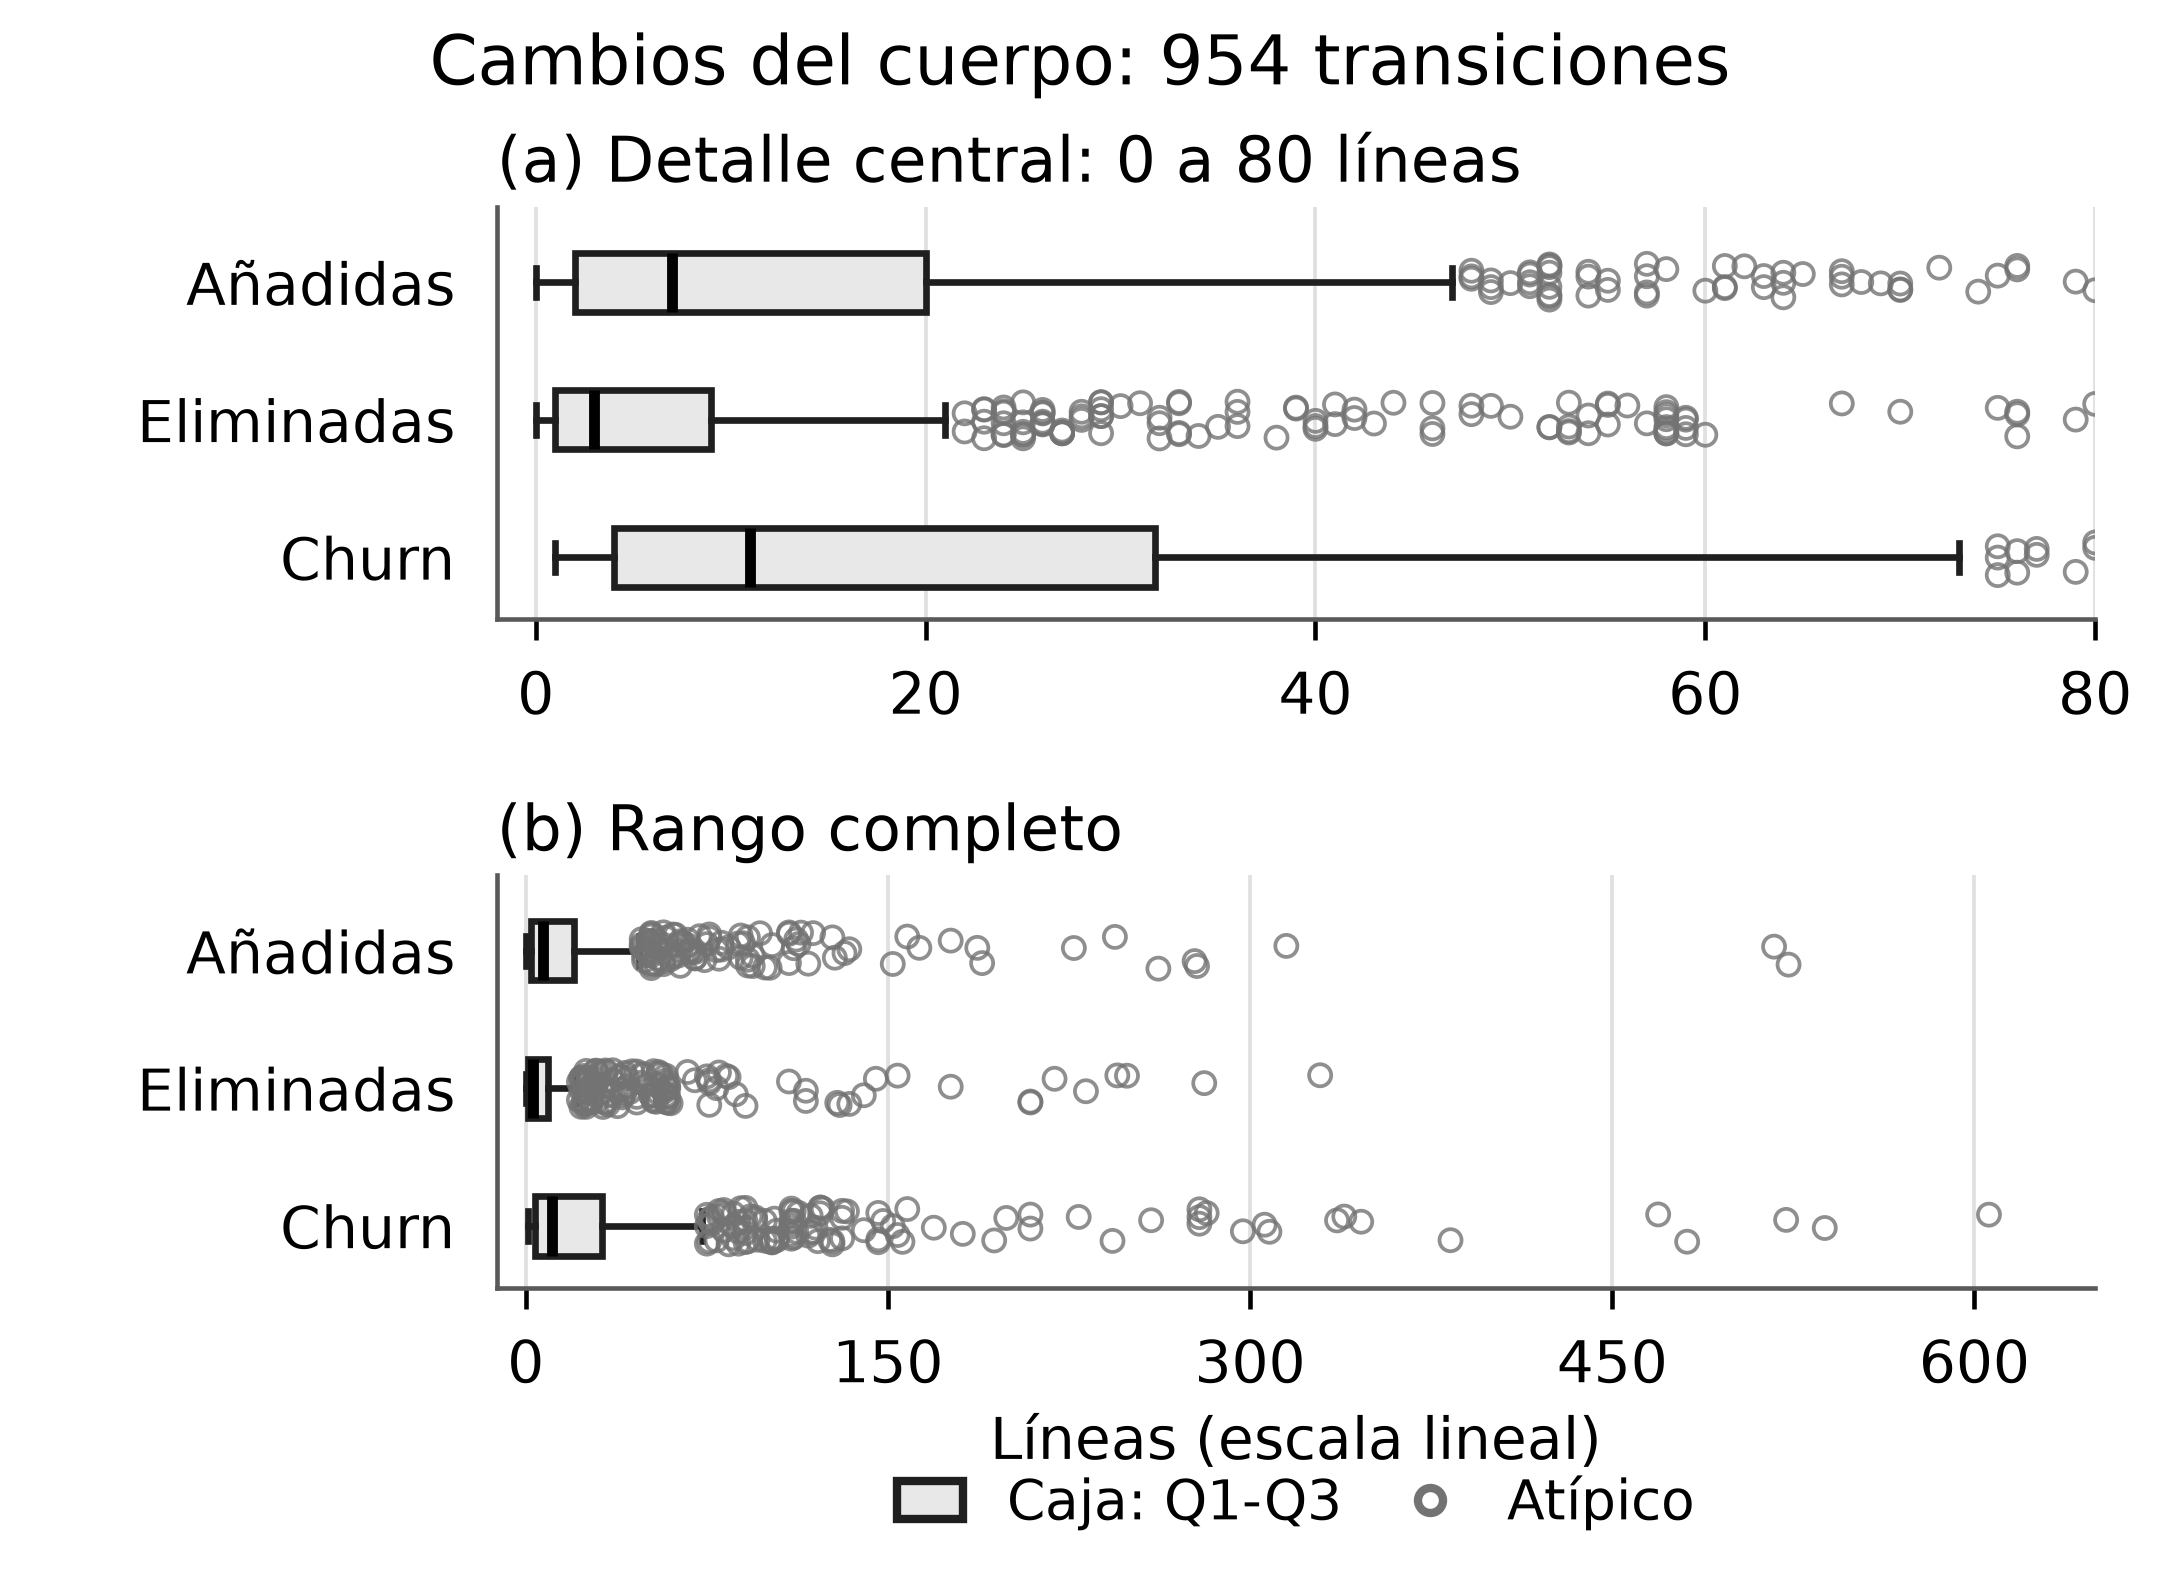
\includegraphics[width=\columnwidth]{figuras/boxplot_cambios.png}
\caption{Líneas añadidas, eliminadas y churn del cuerpo en 954 transiciones efectivas. (a) Detalle de 0 a 80 líneas; (b) rango completo con todos los atípicos. Cajas: $Q_1$--$Q_3$; línea central: mediana; bigotes: regla de $1{,}5\,\mathrm{IQR}$. Los círculos vacíos son valores atípicos.}
\label{fig:churn}
\end{figure}

La Figura~\ref{fig:churn} muestra la cola superior de la distribución: el churn máximo del cuerpo es 606 líneas. En el cuerpo, 579 cambios aumentan el tamaño, 146 lo reducen y 229 lo conservan pese a modificar líneas. Se añadieron 18.388 líneas y se eliminaron 11.190. La mediana de $R$ es 0,086. Las medianas de $A$ y $D$ no se combinan para reconstruir la mediana de $C$.

\subsection{Comparación contextual (RQ3)}
\begin{table}[!ht]
\centering
\caption{Medianas de medianas por repositorio.}
\label{tab:lenguaje}
\footnotesize
\setlength{\tabcolsep}{4pt}
\begin{tabular}{lrrr}
\toprule
Contexto & $N/n$ & $L$ cuerpo & $C$ cuerpo\\
\midrule
TypeScript & 52/33 & 58,25 & 14\\
Go & 41/11 & 1 & 8\\
C\# & 32/25 & 118 & 15\\
Python & 29/17 & 112 & 10,5\\
Makefile & 21/1 & 1 & 4\\
F\# & 18/14 & 225 & 14\\
\bottomrule
\end{tabular}
\par\smallskip
\begin{minipage}{\columnwidth}\footnotesize
$N$: repositorios del contexto; $n$: repositorios con cambios del cuerpo. $L$ usa los $N$ repositorios; $C$ utiliza solo los $n$ con cambios efectivos.
\end{minipage}
\end{table}

\begin{figure}[!ht]
\centering
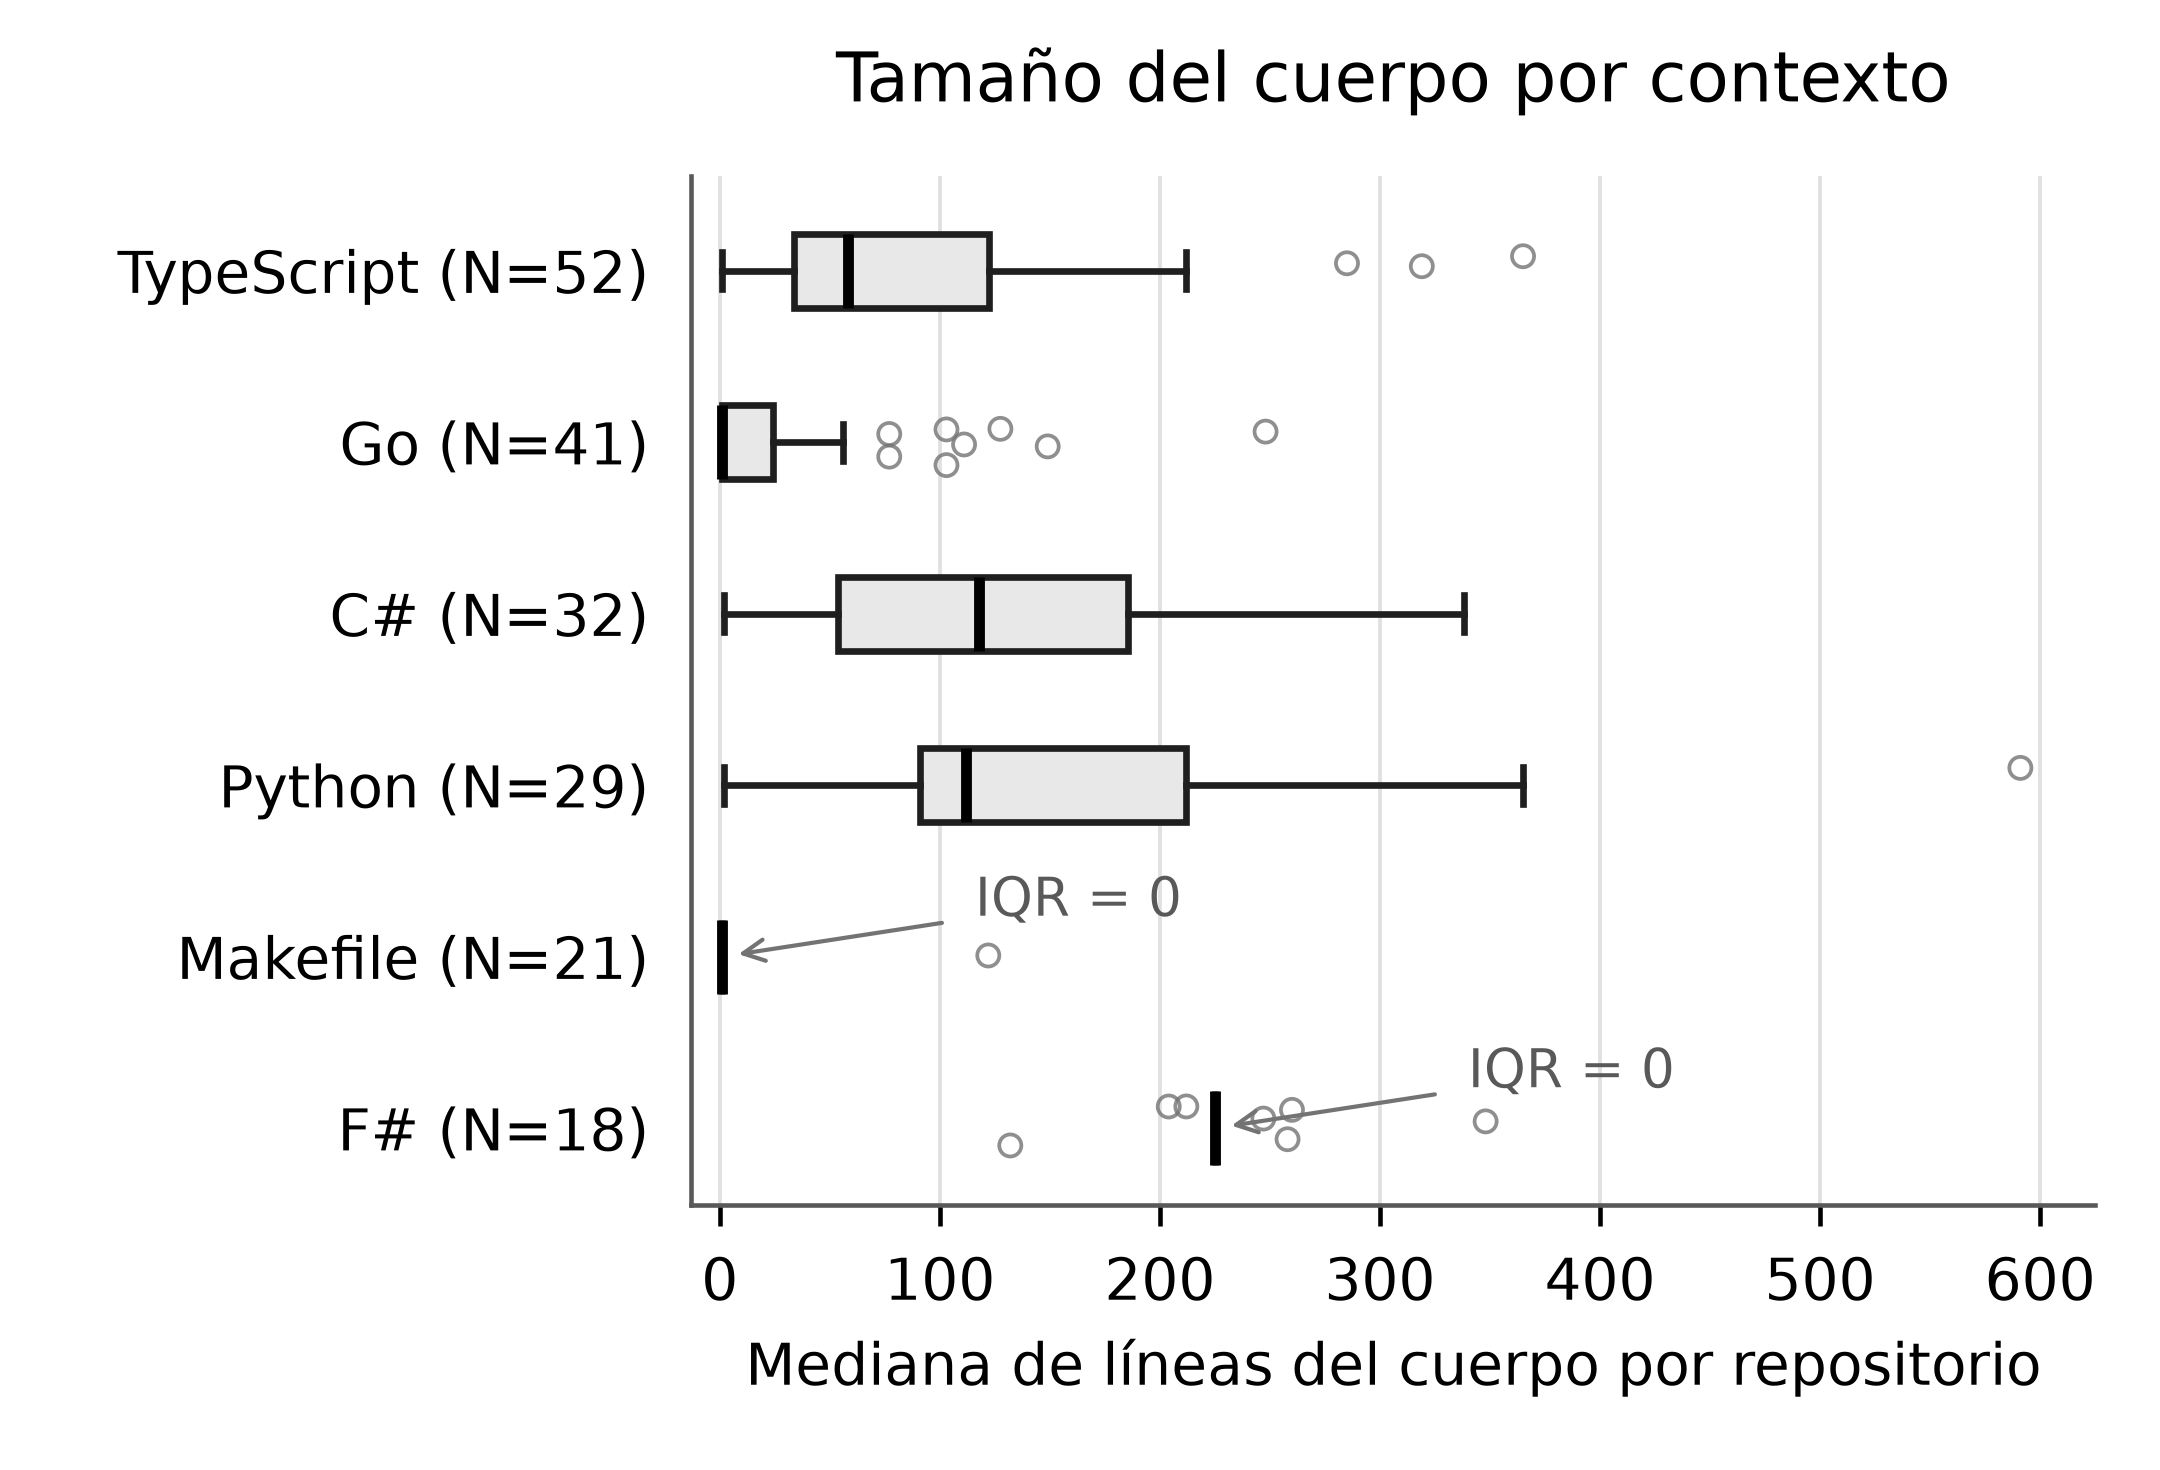
\includegraphics[width=\columnwidth]{figuras/boxplot_lenguajes.png}
\caption{Tamaño del cuerpo por contexto: una mediana de últimas versiones por repositorio. $N$ indica repositorios. Eje lineal y convención de cajas, bigotes y atípicos del método. En Makefile y F\#, $\mathrm{IQR}=0$ y la caja se reduce a una línea.}
\label{fig:lenguaje}
\end{figure}

La Figura~\ref{fig:lenguaje} complementa las medianas con dispersión por contexto. En Makefile y F\#, $Q_1=Q_3$ y la caja se reduce a una línea; los atípicos siguen visibles. Las 96 últimas versiones con cuerpo de una línea usan importaciones; el tamaño local no mide toda la especificación desplegada. Al excluir los 52 repositorios de pulumi, Go queda con 13 repositorios y su mediana pasa de 1 a 77 líneas; el churn mediano permanece en 8. La composición organizacional condiciona la comparación. Makefile tiene solo un repositorio con cambios del cuerpo.

% Fin de la tercera página de contenido prevista.
\clearpage
\section{Limitaciones y amenazas a la validez}
\subsection{Validez de constructo}
Las líneas físicas miden volumen textual, no importancia semántica, claridad, calidad ni esfuerzo. Una reformulación o un cambio de indentación puede elevar $C$ sin modificar el comportamiento. \texttt{SequenceMatcher} es una alineación reproducible, no una medida semántica ni un algoritmo de edición mínima garantizada. Separar cuerpo y YAML reduce la confusión entre instrucciones y configuración, aunque ambos pueden afectar la ejecución.

Las importaciones externas limitan la interpretación del tamaño y de la estabilidad local. Una instrucción importada puede cambiar sin modificar este archivo, y parte de la tarea puede residir en scripts no contenidos en el snapshot. Se detectaron 29 transiciones con diferencias en el texto crudo del cuerpo y $C=0$; no se cuentan como cambios efectivos de líneas. Los boxplots no permiten identificar por sí solos la causa o relevancia de los atípicos.

\subsection{Validez interna y temporal}
El diseño no controla tareas, herramientas, tamaño del proyecto, popularidad ni políticas de mantenimiento. El lenguaje principal de GitHub es un indicador contextual: un repositorio puede ser políglota y etiquetas como Makefile no representan categorías homogéneas. Los archivos estudiados son siempre Markdown. Las asociaciones se interpretan según los límites de observaciones en contextos reales \cite{stol2018}; no se identifica autoría humana o del agente, causa del cambio ni impacto en la ejecución.

Los enlaces y \texttt{rank} describen una secuencia observada, pero no demuestran ramas ni ascendencia Git. Todos los intervalos de las 2.216 transiciones son positivos; esto no prueba historia completa. La mediana entre primera y última versión es 36,26 días en las 406 historias multiversión. Una historia de una versión no prueba falta de mantenimiento posterior. Debido a la censura y a la exposición desigual no se estima una tasa mensual ni una tendencia de estabilización.

\subsection{Validez externa y de las conclusiones}
GHAW-H representa adoptantes tempranos públicos y archivos confirmados mediante locks. No constituye una muestra aleatoria de toda la programación agéntica ni de \texttt{AGENTS.md}. Puede omitir instrucciones, commits y workflows fuera del criterio de selección. \textit{Agent READMEs} fundamenta las dimensiones del diseño; sus hallazgos no son resultados del corpus actual.

Las observaciones de una historia o repositorio están correlacionadas. RQ3 agrega por repositorio, pero subsisten dependencias organizacionales y plantillas: pulumi aporta 52 de los 262 repositorios; las 604 últimas versiones tienen 497 textos completos distintos. Los tamaños de grupos y los subconjuntos con cambios son desiguales. Los boxplots comparan distribuciones descriptivas; su superposición no es una prueba de igualdad ni su separación una prueba de significancia. Una inferencia posterior deberá estudiar sensibilidad a organización, duplicados, importaciones y ventana temporal.

\section{Paquete de réplica y cierre}
El paquete local contiene scripts de descarga y análisis, dependencias, revisión y hashes del dataset, métricas por versión, transición, historia y repositorio, resumen JSON y fuente editable. Las dos figuras se incluyen como imágenes PNG y se regeneran desde los CSV mediante \texttt{scripts/plot\_results.py}; sus estadísticas y atípicos proceden de los datos observados. Los datos crudos se descargan de la revisión fijada y conservan las licencias de sus repositorios de origen.

\noindent\textbf{GitHub del paquete:} \GitHubReplica.\\
\textbf{Zenodo del paquete:} \ZenodoReplica.

Los enlaces propios se incorporarán después de publicar el repositorio y archivar una release. Ambos son requisitos pendientes antes de entregar. El DOI de GHAW-H \cite{ghawh} identifica el dataset de sus autores y no el paquete de este trabajo.

La ejecución preliminar muestra que gran parte de la evolución del archivo corresponde a configuración. En los cambios efectivos del cuerpo, la mediana baja convive con una cola de ediciones extensas. La comparación contextual depende de dónde se almacenan las instrucciones y de la composición de los repositorios. La próxima etapa podrá validar semánticamente una muestra y evaluar esa sensibilidad, sin equiparar volumen textual con calidad del agente.

% Referencias en página separada. Las referencias nuevas se mantienen negras.
\clearpage
\begin{thebibliography}{9}
\bibitem{ghawdocs}
GitHub Next y Microsoft Research, ``Workflow Structure,'' documentación de GitHub Agentic Workflows, consulta: 5 oct. 2026. \url{https://github.github.io/gh-aw/reference/workflow-structure/}.

\bibitem{stol2018}
K.-J. Stol and B. Fitzgerald, ``The ABC of Software Engineering Research,'' \textit{ACM Trans. Softw. Eng. Methodol.}, vol. 27, no. 3, 2018, art. 11. \url{https://doi.org/10.1145/3241743}.

\bibitem{agentreadmes}
W. Chatlatanagulchai et al., ``Agent READMEs: An Empirical Study of Context Files for Agentic Coding,'' preprint, arXiv:2511.12884v2, 9 ago. 2026. \url{https://arxiv.org/abs/2511.12884v2}.

\bibitem{jiang2026}
S. Jiang and D. Nam, ``Beyond the Prompt: An Empirical Study of Cursor Rules,'' \corr{preprint, arXiv:2512.18925v3, 4 mar. 2026}. \url{https://arxiv.org/abs/2512.18925v3}.

\bibitem{easterbrook2008}
S. Easterbrook, J. Singer, M.-A. Storey, and D. Damian, ``Selecting Empirical Methods for Software Engineering Research,'' in \textit{Guide to Advanced Empirical Software Engineering}, Springer, 2008, pp. 285--311. \url{https://doi.org/10.1007/978-1-84800-044-5_11}.

\bibitem{ghawh}
P. Valenzuela-Toledo, T. Kehrer y S. Panichella, ``GHAW-H: A Dataset of GitHub Agentic Workflow Histories,'' v0.1.2, Zenodo, 2026. \url{https://doi.org/10.5281/zenodo.22084012}.
\end{thebibliography}
\end{document}
